\documentclass[tikz,border=2pt]{standalone}
\usepackage{pgfplots}
\pgfplotsset{compat=1.7}

\begin{document}
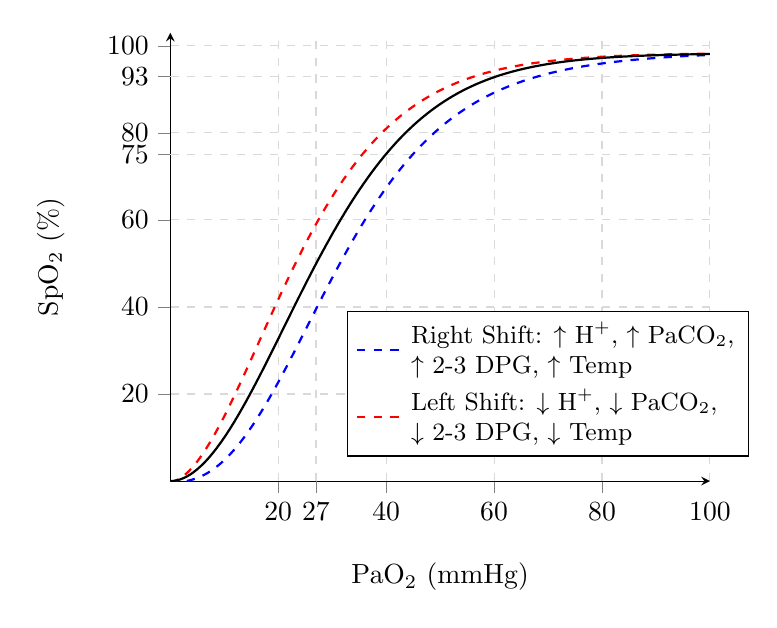
\begin{tikzpicture}

\tikzset{
    myarrow/.style={
        sloped,
        isosceles triangle,
        anchor=apex,
        fill=black,
        inner sep=2pt
    }
}
    \begin{axis}[
        axis lines=middle,
	ymin = 0,
	ymax = 103,
	xmin = 0,
xmax = 100,
        grid = major,
        grid style={dashed, gray!30},
	 ylabel near ticks,
	xlabel near ticks,
		extra x ticks={27},
	extra x tick labels = {27},
		extra y ticks={75,93},
	extra y tick labels = {75,93},
        xlabel=PaO\textsubscript{2} (mmHg),
        ylabel=SpO\textsubscript{2} (\%),
        tick align=outside,
        enlargelimits=false,
	legend pos = south east,
legend style={font=\small, cells={align=left}, at={(0.7,0.38)},anchor=north},
legend cell align={left}]

	\addplot[domain=0:100, blue, thick, dashed,samples=500] {98.92857 + (-0.2890872 - 98.92857)/(1 + (x/50.75804)^2.379558)^2.549376};
	\addlegendentry{Right Shift: $\uparrow$ H\textsuperscript{+}, $\uparrow$ PaCO\textsubscript{2}, \\ $\uparrow$ 2-3 DPG, $\uparrow$ Temp};
	\addplot[domain=0:100, red, thick, dashed,samples=500] {98.43243 + (-0.1346508 - 98.43243)/(1 + (x/76.70556)^1.784125)^6.355281};
	\addlegendentry{Left Shift: $\downarrow$ H\textsuperscript{+}, $\downarrow$  PaCO\textsubscript{2}, \\ $\downarrow$  2-3 DPG, $\downarrow$  Temp};
	\addplot[domain=0:100, black, thick,samples=500] {98.32157 + (-0.008578349 - 98.32157)/(1 + (x/90.23375)^1.937563)^7.691635};
\end{axis}

\end{tikzpicture} 
\end{document}